%% img/complexity_intro/HAMPATHCYCLE.tex
%% Copyright 2019 Andrea Berlingieri
%
% This work may be distributed and/or modified under the
% conditions of the LaTeX Project Public License, either version 1.3
% of this license or (at your option) any later version.
% The latest version of this license is in
%   http://www.latex-project.org/lppl.txt
% and version 1.3 or later is part of all distributions of LaTeX
% version 2005/12/01 or later.
%
% This work has the LPPL maintenance status `maintained'.
%
% The Current Maintainer of this work is Andrea Berlingieri.
%
% This work consists of all files listed in manifest.txt
\documentclass{standalone}

\usepackage{../TikzStyle}
\usepackage{../mystyle}

\begin{document}
    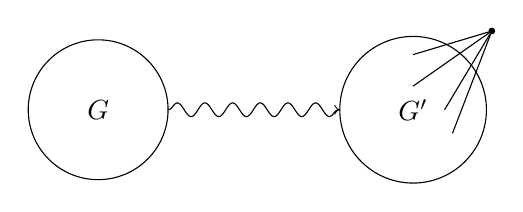
\begin{tikzpicture}
        \node[draw,circle,inner sep=0.5cm] (G) at (0,0) {$G$};
        \node[draw,circle,inner sep=0.5cm] (G1) at (4,0) {$G'$};
        \draw[->,decorate,decoration=snake] (G) -- (G1);
        \node[draw,circle,inner sep=0cm,fill=black,minimum size=2pt] (n) at (5,1) {};
        \draw (n) -- (4,0.3);
        \draw (n) -- (4,0.7);
        \draw (n) -- (4.4,0);
        \draw (n) -- (4.5,-0.3);
    \end{tikzpicture}
\end{document}
